\RequirePackage[l2tabu, orthodox]{nag}
\documentclass{article}
%%% use this declaration to set specific page margins %%%
\usepackage[a4paper, lmargin = {1.5cm}, rmargin = {1.5cm}, tmargin = {1.5cm}, bmargin = {1.5cm}]{geometry}
%\usepackage[a4paper]{geometry}
%\usepackage[titletoc]{appendix}

%\usepackage[ngerman, english]{babel}
\usepackage[fontsize=10pt]{scrextend}
\usepackage[utf8]{inputenc}
\usepackage[numbers]{natbib}
\usepackage[default]{lato}
\usepackage[T1]{fontenc}
% \usepackage[latin1]{inputenc}                    % german characters
\usepackage{graphicx}                              % it's recommended to use PDF images but you can use JPG or PNG as well
\usepackage{url}                                   % format URLs
\usepackage{hyperref}                              % create hyperlinks
\usepackage{listings, color}                       % for source code
%\usepackage{subfig}                               % two figures next to each other (example: figure 3a), figure 3b)
%\usepackage{csquotes}
%\usepackage{amsmath}
\usepackage{array}
\usepackage{microtype}
\usepackage{enumitem}
\usepackage{verbatim}
\usepackage{multirow}

%%% page numbering %%%
\usepackage{fancyhdr}
\usepackage[page]{totalcount}
\usepackage{lastpage}
\pagestyle{fancy}
\pagenumbering{arabic}
\fancyhf{} % clear all header and footer fields
\fancyhead[L]{https://github.com/qqzhong/sort}
\fancyhead[C]{Page \thepage \hspace{1pt} of \totalpages}
\fancyhead[R]{Internal Document}
\fancyhead[L]{https://github.com/qqzhong/sort}
\fancyfoot[C]{Page \thepage \hspace{1pt} of \totalpages}
\fancyfoot[R]{Internal Document}
\renewcommand{\headrulewidth}{0.5pt}
\renewcommand{\footrulewidth}{0.5pt}


%%% insert code %%%
\usepackage{listings}
\usepackage{color}

\definecolor{dkgreen}{rgb}{0,0.6,0}
\definecolor{gray}{rgb}{0.5,0.5,0.5}
\definecolor{mauve}{rgb}{0.58,0,0.82}

% language=C
\lstset{frame=single,
  aboveskip=3mm,
  belowskip=3mm,
  showstringspaces=false,
  columns=flexible,
  basicstyle={\small\ttfamily},
  numbers=none,
  numberstyle=\tiny\color{gray},
  keywordstyle=\color{blue},
  commentstyle=\color{dkgreen},
  stringstyle=\color{mauve},
  breaklines=true,
  breakatwhitespace=true,
  tabsize=2
}


%%% document %%%
\begin{document}


%%% title of this paper %%%
\begin{titlepage}
	\vspace*{\stretch{1.0}}
	\begin{center}
		\Large\textbf{"Low Disk Space" issue of rootfs on the 16MB Flash}\\
		\vspace{1.0cm}
		\large\textsf{Church.ZHONG}\\
		\vspace{1.0cm}
		\large\textsf{535455233@qq.com}\\
		\vspace{1.0cm}
		\large\textsf{\today}
	\end{center}
	\vspace*{\stretch{2.0}}
\end{titlepage}

\setlength{\parindent}{20pt}

\section{Issue Description}

\textbf
After new firmware was released, QA engr reports an issue that the size of free disk decreases 1MB.

\textbf
"This is terrible. It's Low Disk Space issue. It's time to make the difference.", so I said.
But firstly I need find out which file size increases significantly for the new firmware revision.

\textbf
So I have to comapre all files one by one between the new firmware and last healthy firmware.
Yes, the "disk space killer" is found and the issue is fixed soon.

\textbf
"How to effectively solve or prevent this kind of Low Disk Space issue?" I have to think about it.
After lunch, I capture some instant ideas to make a common tool to find "disk space killer".

\textbf
OK, let's try them.


\section{A Root Cause Analysis (RCA) Tool}

\textbf
Assume that we have 4 files in firmware:


\begin{lstlisting}[language={[ansi]C}]
android@Church:/latex/amazon/rootfs$
-rw-rw-r-- 1 android android  5632 Aug 29 10:45 file0.txt
-rw-rw-r-- 1 android android 51712 Aug 29 10:45 file1.txt
-rw-rw-r-- 1 android android 52224 Aug 29 10:46 file2.txt
-rw-rw-r-- 1 android android 52736 Aug 29 10:46 file3.txt
    \end{lstlisting}


\textbf
And generate the firmware revision A001 by command "tar -zcf firmware\_A001.tgz rootfs/".


\textbf
But then we add something(maybe add new feature or modify something to fix bugs) into the firmware:


\begin{lstlisting}[language={[ansi]C}]
android@Church:/latex/amazon/rootfs$
-rw-rw-r-- 1 android android  10752 Aug 29 10:52 file0.txt
-rw-rw-r-- 1 android android 102912 Aug 29 10:52 file1.txt
-rw-rw-r-- 1 android android 103424 Aug 29 10:52 file2.txt
-rw-rw-r-- 1 android android 103936 Aug 29 10:52 file3.txt
    \end{lstlisting}

\textbf
And generate the firmware revision A002 by command "tar -zcf firmware\_A002.tgz rootfs/".

\textbf
We can notice that all files(file0,file1,file2,file3) in firmware revision A002 are greater than files in firmware revision A001.

\textbf
But now we have to comapre all files one by one between the firmware revision A001 and A002 if we want to find the "disk space killer".

\textbf
It will be tough and difficult to find the "disk space killer" if there are a large of files in firmware.

\textbf
Usually we can get the shopping detailed list after finished payment in supermarket.

\textbf
Similarly, it is likewise smart("SMART") to generate the rootfs report for the firmware while releasing the new firmware.

\textbf
We can write a script tool of python/perl/golang/bash to improve it.

\textbf
Here I take bash/awk as our example.

\textbf
OK, let's do it.

    
\textbf
We can get file size and file name after run command "du -a -b ./rootfs":

    
\begin{lstlisting}[language={[ansi]C}]
android@Church:/latex/amazon$ du -a -b ./rootfs
103936	../rootfs/file3.txt
103424	../rootfs/file2.txt
10752	../rootfs/file0.txt
102912	../rootfs/file1.txt
325120	../rootfs
    \end{lstlisting}

\textbf
And we can sort the above output by command "sort.awk":

\begin{lstlisting}[language={[ansi]C}]
android@Church:/latex/amazon$ du -a -b ./rootfs > output.txt
android@Church:/latex/amazon$ ./sort.awk output.txt
./rootfs/file3.txt,103936
./rootfs/file2.txt,103424
./rootfs/file1.txt,102912
./rootfs/file0.txt,10752
    \end{lstlisting}

\textbf
So we can gte the firmware report by command "./sort.awk output.txt > report.txt".


\textbf
Below is the whole content of file "sort.awk":


\begin{lstlisting}[language={bash}]
#!/usr/bin/awk -f

{
	cmd=sprintf("test -f %s",$2);
	f=system(cmd);
	n++;
	if(0==f)
	{
		# pack line by line
		data[n]=sprintf("%32s%s,%s",$1,$2,$1);
	}
	# skip all directories
}
END{
	# sort in decreasing order line by line
	m=asort(data);
	for(i=m;i>=1;i--)
	{
		# unpack line by line
		print substr(data[i],33);
	}
}
    \end{lstlisting}

It is easy to get the reports of the firmware revision A001 and A002:
\begin{lstlisting}[language={[ansi]C}]
du -a -b ./rootfs_R001 > output_R001.txt
./sort.awk output_R001.txt > report_R001.txt

du -a -b ./rootfs_R002 > output_R002.txt
./sort.awk output_R002.txt > report_R002.txt
    \end{lstlisting}


\textbf
At last, we can compare the report\_R001.txt and report\_R002.txt:
\begin{figure}[h]
	\centering
	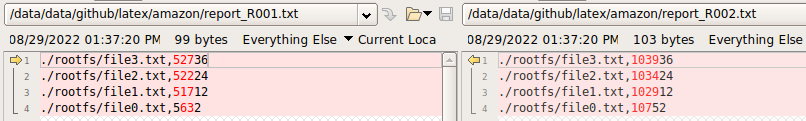
\includegraphics[scale=0.5]{report.png}
	\caption{compare the reports by beyond compare}
	\label{fig:label}
\end{figure}


\section{How to make smaller firmware}

\textbf
There are some useful optimization flags for C language to make smaller firmware:

\textbf
1) Remove dead codes and unused legacy codes from the project.

\textbf
2) Use -s to strip debug info from the binary (and don't use -g).

\textbf
3) Use -Os to optimize for output file size.

\textbf
4) Use -ffunction-sections -fdata-sections to separate each function or data into distinct sections within the translation unit. Combine it with the linker option -Wl,--gc-sections to get rid of any unreferenced sections.


\section{Make further efforts}

\textbf
With Continuous Integration (CI) widely used and Gerrit and Jenkins ecosystem matured, the DevOps engr can easily develop the rootfs size checker tool for the Gerrit and Jenkins.

\textbf
Then, we can imagine below workflows about "CI".

\textbf
1) Assume that the latest firmware revision is A001 and the rootfs report revision is R001 and the rootfs is healthy.

\textbf
2) A software engineer changes codes then push to Gerrit server, then Jenkins server build new firmware(A002) and new rootfs report(R002). But the rootfs size checker find "Low Disk Space" issue again after compared the rootfs report R001 and R002.

\textbf
3) Oops, the software engineer must check codes and find why rootfs free space becomes lower.

\textbf
Yes, the rootfs size checker (and the rootfs sort tool) and this "CI" workflows both come true in my experience.


\section{What can we learn}

\textbf
Here'are some my thoughts:

\textbf
1) Don't ignore small problems. Solve them before they become huge problems.


\textbf
2) Turning brainstorming into action. Open source is powerful and always remember that we're "On the Shoulders of Giants."
we can write scripts or demonstrations to speed up the validation process.


\end{document}

